
%% LaTeX Beamer presentation template (requires beamer package)
%% see http://bitbucket.org/rivanvx/beamer/wiki/Home
%% idea contributed by H. Turgut Uyar
%% template based on a template by Till Tantau
%% this template is still evolving - it might differ in future releases!

% \documentclass[draft]{beamer}
% \documentclass[handout]{beamer}
\documentclass{beamer}
% \usepackage{pgfpages} %for two screen presentations
% \pgfpagesuselayout{2 on 1}[a4paper,border shrink=5mm] %for handout!
% \setbeameroption{show notes} 
% \setbeameroption{show notes on second screen}
% \setbeameroption{show next slide on second screen}
% \setbeameroption{second mode text on second screen=left}
\setbeamertemplate{navigation symbols}{}

\mode<presentation> 
{
\usetheme{Warsaw} 
% \usetheme{Frankfurt}
% \usetheme{Berkeley}
\usecolortheme{seahorse}
% \usecolortheme{rose}
\usefonttheme[onlylarge]{structuresmallcapsserif}
\usefonttheme[onlysmall]{structurebold}

\setbeamercovered{transparent}
\setbeamercolor{title}{fg=blue!90!black,bg=red!70!white}
}

\usepackage[english]{babel}
\usepackage[latin1]{inputenc}

% font definitions, try \usepackage{ae} instead of the following
% three lines if you don't like this look
\usepackage{mathptmx}
\usepackage[scaled=.90]{helvet}
\usepackage{courier}

\usepackage[T1]{fontenc}

\usepackage{amsmath}
\usepackage{amscd}
\usepackage{amssymb}
\usepackage{amsfonts}
\usepackage{amsthm}
\usepackage{amsfonts}
\usepackage{amsthm}

\usepackage{tikz}
\usepackage{subcaption}
\usepackage{subfigure}

\usepackage{aviolov_style}
\usepackage{local_style}


\title[Opt-Design for SDEs]
{Optimal Design for Stochastic Differential Equations}
% - Use the \inst{?} command only if the authors have different
%   affiliation.
\author{Alexandre Iolov}
% \institute{Annual Meeting in the Statistics Network, Holte}
\date{Feb 3rd, 2014}
% % This is only inserted into the PDF information catalog. Can be left
% % out.
% \subject{Talks}
% If you have a file called "university-logo-filename.xxx", where xxx
% is a graphic format that can be processed by latex or pdflatex,
% resp., then you can add a logo as follows:
% \pgfdeclareimage[height=0.5cm]{university-logo}{university-logo-filename}
% \logo{\pgfuseimage{university-logo}}
% Delete this, if you do not want the table of contents to pop up at
% the beginning of each subsection:
% \AtBeginSubsection[]
% {
% \begin{frame}<beamer>
% \frametitle{Outline}
% \tableofcontents[currentsection,currentsubsection]
% \end{frame}
% }

% If you wish to uncover everything in a step-wise fashion, uncomment
% the following command:
%\beamerdefaultoverlayspecification{<+->}

\begin{document}

\begin{frame}
\titlepage
\end{frame}

% \section*{Outline}
\begin{frame}
\tableofcontents[pausesections]
\end{frame}

\section{Problem Background - Parametrized SDEs and Mutual Information}  
\begin{frame}
\frametitle{The Basic Setup} 
% \framesubtitle{Subtitles are optional}
Consider  
% \begin{center}
a parametrized SDE:
\begin{equation*}
\begin{gathered}
dX = U(x,\a(x,t); \th) \intd{t} + \sqrt{2D} dW
\\
\th \sim \textrm{Unknown parameters (in the drift)}
\\
\a \sim \textrm{External perturbation}
\end{gathered}
\end{equation*}
\\
\onslide<2-3> {
 For example the 'double-well potential':
\begin{equation*}
\begin{gathered}
dX = \underbrace{ -\left( 4x^3 - 4x -A \frac xc e^{-(x/c)^2/2} \right) +
\a(x,t)}_{U(x,\a; \th)} \intd{t} + \sqrt{2D} dW
\\
\th \sim \{A\} \quad \textrm{ the barrier height}
\end{gathered}
\end{equation*}
}
% \end{center}
\onslide<3>{
ASSUMPTION: 'continuous' observations of the trajectories $X_t$.
}
\end{frame}

\begin{frame}
\frametitle{Our Goal}
Choose $\a(x,t)$ so as to facilitate the estimation of the unknown parameters,
$\th$.
\begin{figure}
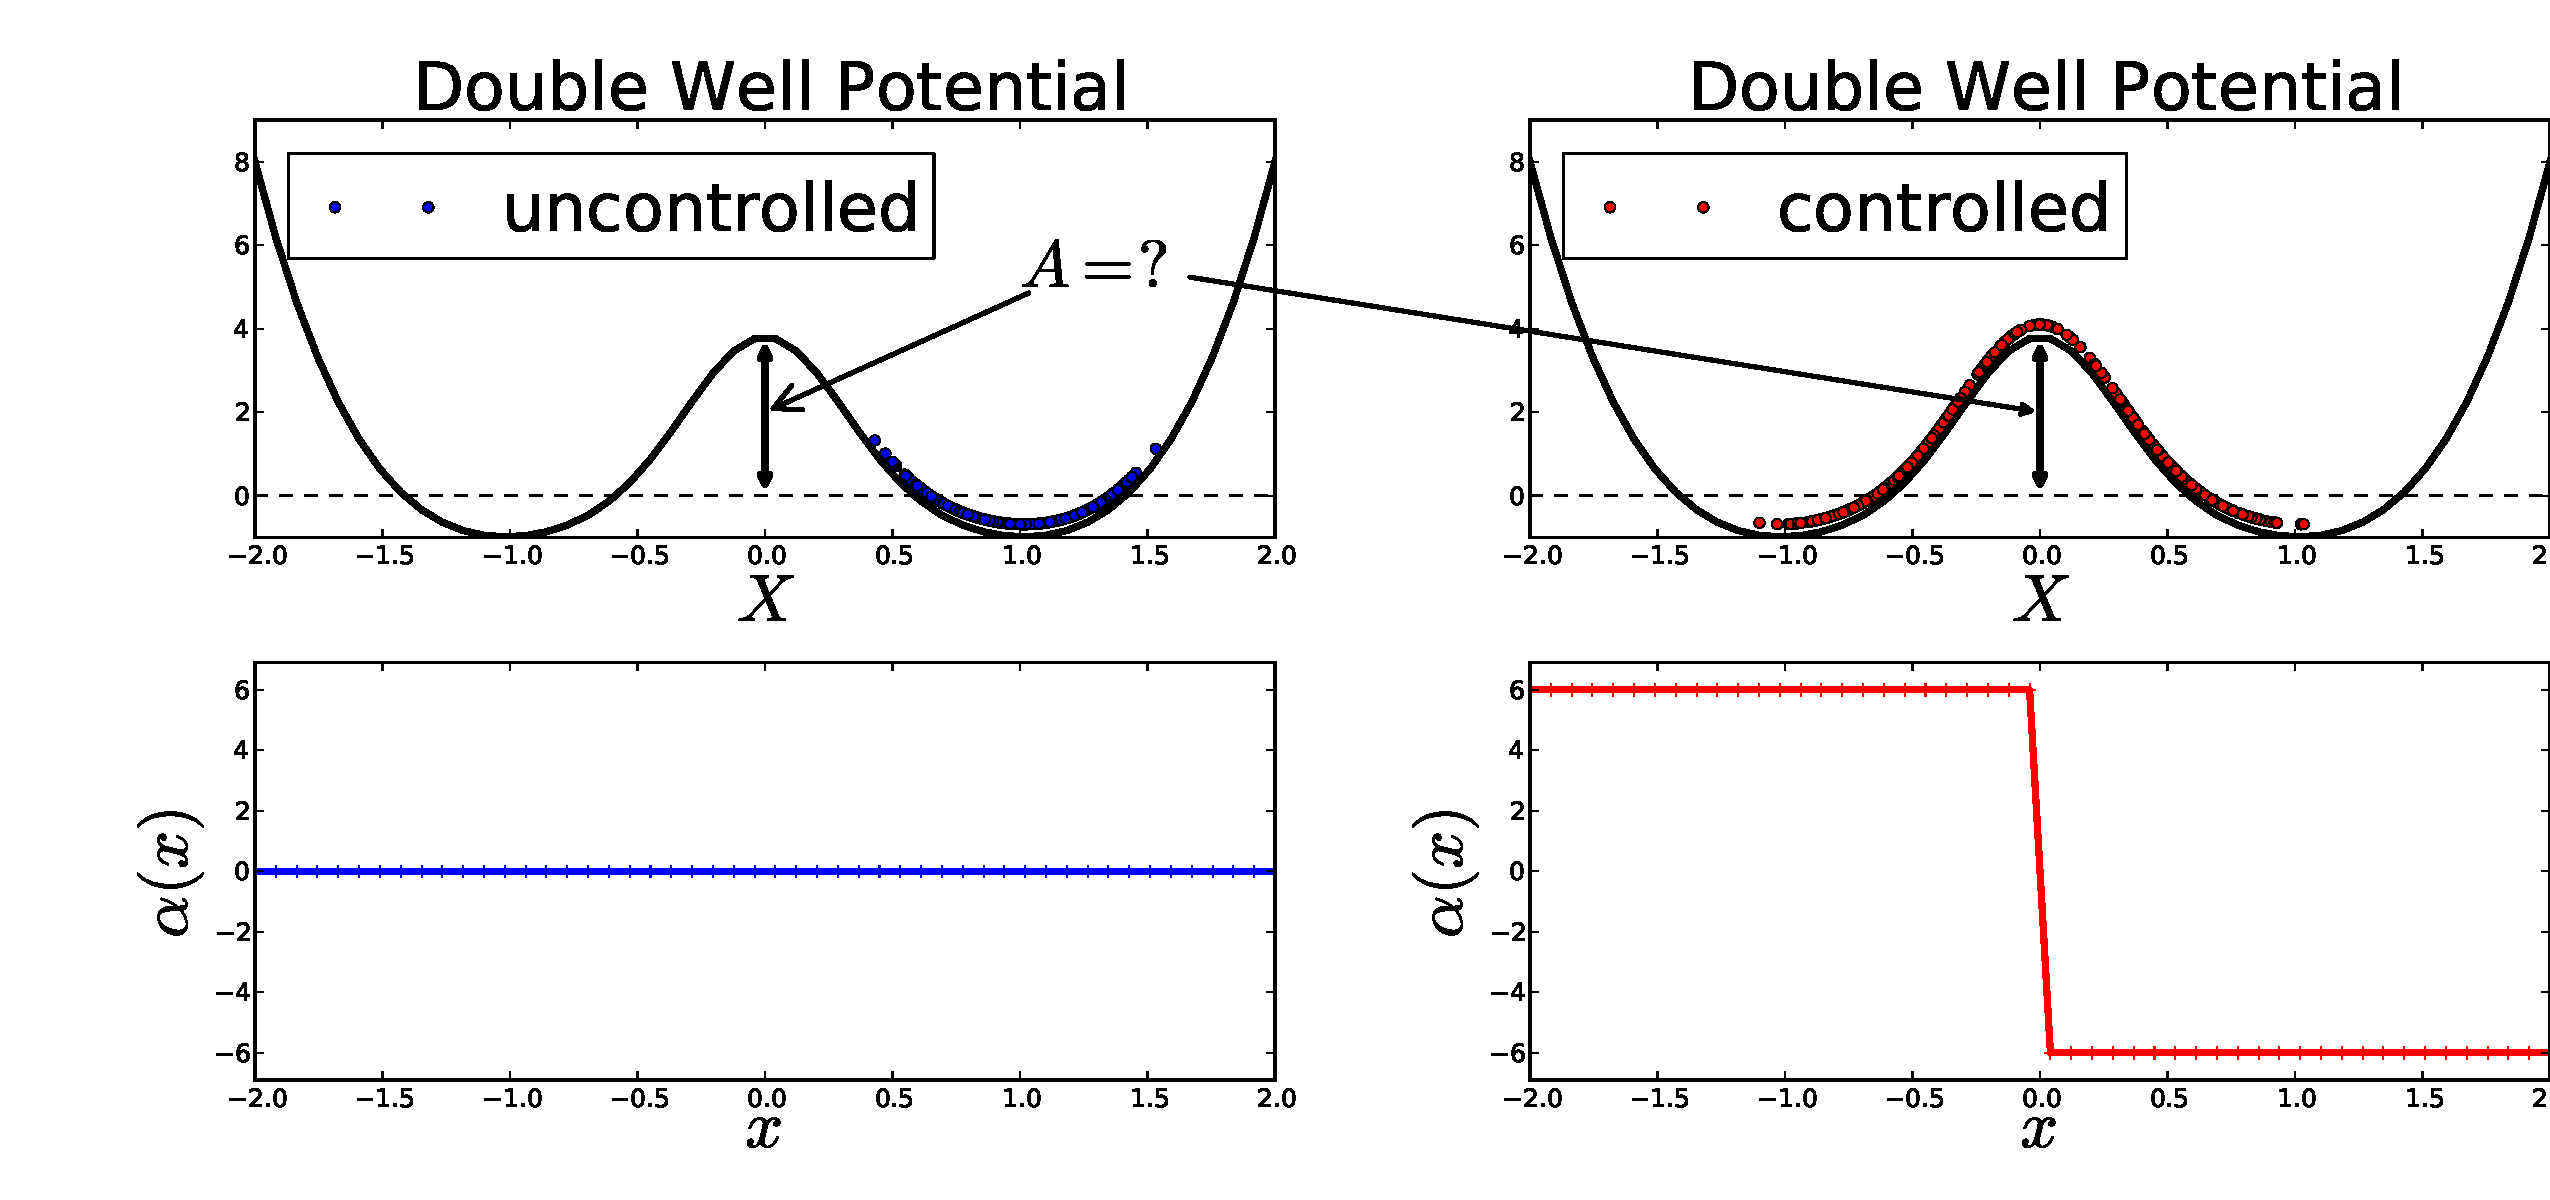
\includegraphics[width=0.99\textwidth]
{Figs/Simulator/doublewell_example_trajectory.pdf}
\end{figure}

\end{frame}
  
\begin{frame}
\frametitle{Formalizing the Goal}
Key Concepts:
\begin{itemize}
  \item Mutual Information between two Random Variables, $I(\th, X)$
  \item Belief Distribution (prior) on the parameters, $\rho(\th)$ 
  \item The transition density of the state, $f(x,t | \th)$
\end{itemize}
\end{frame} 
\begin{frame}
\frametitle{Mutual Information - Definition}
For a given control, $\a(x,t)$, the Mutual Information, $I$ between the R.V.s
$X,\th$ is:
\begin{eqnarray*}
I(X,\th) &=& \int_\Theta \int_X p(x,\th) \cdot \log \left(
\frac{p(x,\th)}{p(x)p(\th)}\right) \intd{x} \intd{\th}
\\
&=& \int_\Theta \int_X 
\log \left( \frac{L(x|\th)  }
				 {\int_\Theta L(x|\th)
\rho(\th)  \intd{\th}} \right)
\cdot
 \underbrace{L(x|\th)}_{\textrm{likelihood}}\underbrace{\rho(\th)}_{\textrm{prior}} 
\intd{x}\intd{\th}
\end{eqnarray*}
\pause
But
\begin{eqnarray*}
L(x,\th) =& \prod_k f(x_k | x_{k-1}) 
\end{eqnarray*}
and
 \begin{eqnarray*}
	dx = \prod {dx_k}
 \end{eqnarray*} 
\pause
(My) conclusion: With multi-observations, $I(X,\th)$ is intractable.
\end{frame} 


\begin{frame}
\frametitle{Single Slice Mutual Information}
For a single observation, however, the Mutual Information is tractable
\begin{eqnarray*}
I(X_t,\th) &=& 
\int_\Theta \int_{\O_X} 
\log \left( \frac{f(x,t| x_0; \th ; \a(\cdot) ) }
				 {\int_\Theta f(x,t| x_0; \th ; \a(\cdot) )
\cdot \rho(\th) \intd{\th} } \right)
\cdot \\&&
\quad \quad \quad  f(x,t| x_0; \th ; \a(\cdot) ) \rho(\th) 
\intd{x}\intd{\th}
\end{eqnarray*}
\onslide<2>{
Time out!
\begin{equation*}
\underbrace{f}_{\textrm{Prob. that}}(\underbrace{x,t}_{X_t=x}
\underbrace{|}_{\textrm{given}}
\underbrace{x_0}_{X_0 = x_0};
\underbrace{\th}_{\textrm{params}} ;
\underbrace{\a(\cdot)}_{\textrm{applied control}} )
\end{equation*}
}
\onslide<3>{
Natural next step, integrate $I$ over time to form the objective $J$:
\begin{eqnarray*}
J[ \a(\cdot)]  &=& \int_0^T I(X_t, \th)\intd{t}
\\
\a^*(x,t) &=& \argmax_{\a(\cdot)} J[ \a(\cdot)] 
\end{eqnarray*}
}

\end{frame}

\begin{frame}
\frametitle{Integrated Single-Slice Mutual Information as the Objective}
\begin{block}{Formal Problem Statement}
Given, $\rho(\th), T$, find
\begin{eqnarray*}
\a(x,t) = \argmax_{\a(x,t)} \Big\{ \, J[\a] =
\int_{\Theta}
\int_{0}^T 
\int_{\O_X}& 
\log \left( \frac{f(x,t|\th) }
				 {\int_\Theta f(x,t|\th)
\cdot \rho(\th) \intd{\th} } \right) \cdot
\\&
  f(x,t| \th) \rho(\th) 
\intd{x} \intd{t} \intd{\th}
  \Big\}
\end{eqnarray*}
\end{block}
\end{frame}

\begin{frame}
You can also write the objective $J$ as

\begin{eqnarray*}
J[\a]&  =& 
\int_{\Theta}
\int_{0}^T 
\int_{\O_X} 
\log \left( \frac{f(x,t|\th) }
				 {\int_\Theta f(x,t|\th)
\cdot \rho(\th) \intd{\th} } \right) \cdot
  f(x,t| \th) \rho(\th) 
\intd{x} \intd{t} \intd{\th}
\\
& =&  \Exp_{\th} \Bigg[
\Exp_{X_t|\th; \a(\cdot)}
\left[ \int_0^T \log\left(\frac{f(X_t,t|\th; \a(\cdot))}
{\int_\th f(X_t,t|\th; \a(\cdot)) \rho(\th)\intd{\th}}\right) \intd{t} \right]
\Bigg] 
\end{eqnarray*}

\pause
Unfortunately, I don't see how to apply Dynamic Programing to this.
\end{frame}
 
\section{Maximizing the Mutual Information using the Adjoint Method for
PDEs}
\begin{frame}
\frametitle{Maximum Principle Solution}
Treat the maximization of $J$ as an Optimization Problem over
Partial Differential Equations (PDEs)
\vskip 10pt
Recall that the transition density, $f(x,t|)$ satisfies a Fokker-Planck (Forward
Kolmogorov) PDE:
\begin{eqnarray*}
\di_t f 
&=&
 D \cdot \di_x^2 [f] - \di_x[U(x,\a(x,t); \th) \cdot f]
\\
&=& \L_{\th, \a(\cdot)}[f]
\end{eqnarray*}

\end{frame} 
\begin{frame}
\frametitle{Maximum Principle Solution}
ROUGH, HAND-WAVY EXPLANATION OF WHAT THE MAXIMUM PRINCIPLE (ADJOINT METHOD) DOES

\pause
\vskip 10pt
\begin{eqnarray*}
J[\a]&  =& 
\Exp_\th \Bigg[ 
\int_{0}^T 
\int_{\O_X} 
\log \left( \frac{f(x,t|\th) }
				 {\int_\Theta f(x,t|\th)
\cdot \rho(\th) \intd{\th} } \right) \cdot
  f(x,t| \th) 
\intd{x} \intd{t} \Bigg]
\end{eqnarray*}
\end{frame} 

\begin{frame}
\begin{eqnarray*}
\di_t \ft  
&=& \L_{\th, \a(\cdot)}[\ft]
\\
-\di_t \pt &=& 
\Lstar_{\th;\a} [p_\th] +   
1 - \frac{  w_\th \ft }{\sum_\th w_\th\ft} 
+ \log\left(\frac{f_\th} {\sum_\th \wt \ft }\right)   
\end{eqnarray*}
And once $\pt, \ft$ are solved for, the differential wrt.\ $\a$ comes
out to:
$$
\frac {\delta J}{\delta \a} \Big|_{x,t} = \sum_\theta \wt  \Big[\di_x \pt(x,t) \cdot
\ft(x,t) \Big] $$

\vskip 10pt

where, for simplicity, the parameters' belief distribution, $\rho(\th)$ has
been discretized: 
$$
\Exp_\th[\cdot] = \int_\Theta [\cdot ] \rho(\th)\intd{\th} \approx \sum_\th\wt 
[\cdot] $$
\pause


\end{frame}
\section{Illustrative Example - the Double Well Potential} 
\begin{frame}
% \frametitle{A more fair comparison}
\frametitle{Back to the Double-Well Potential} 
\begin{figure}[htp] 
\begin{center}  
  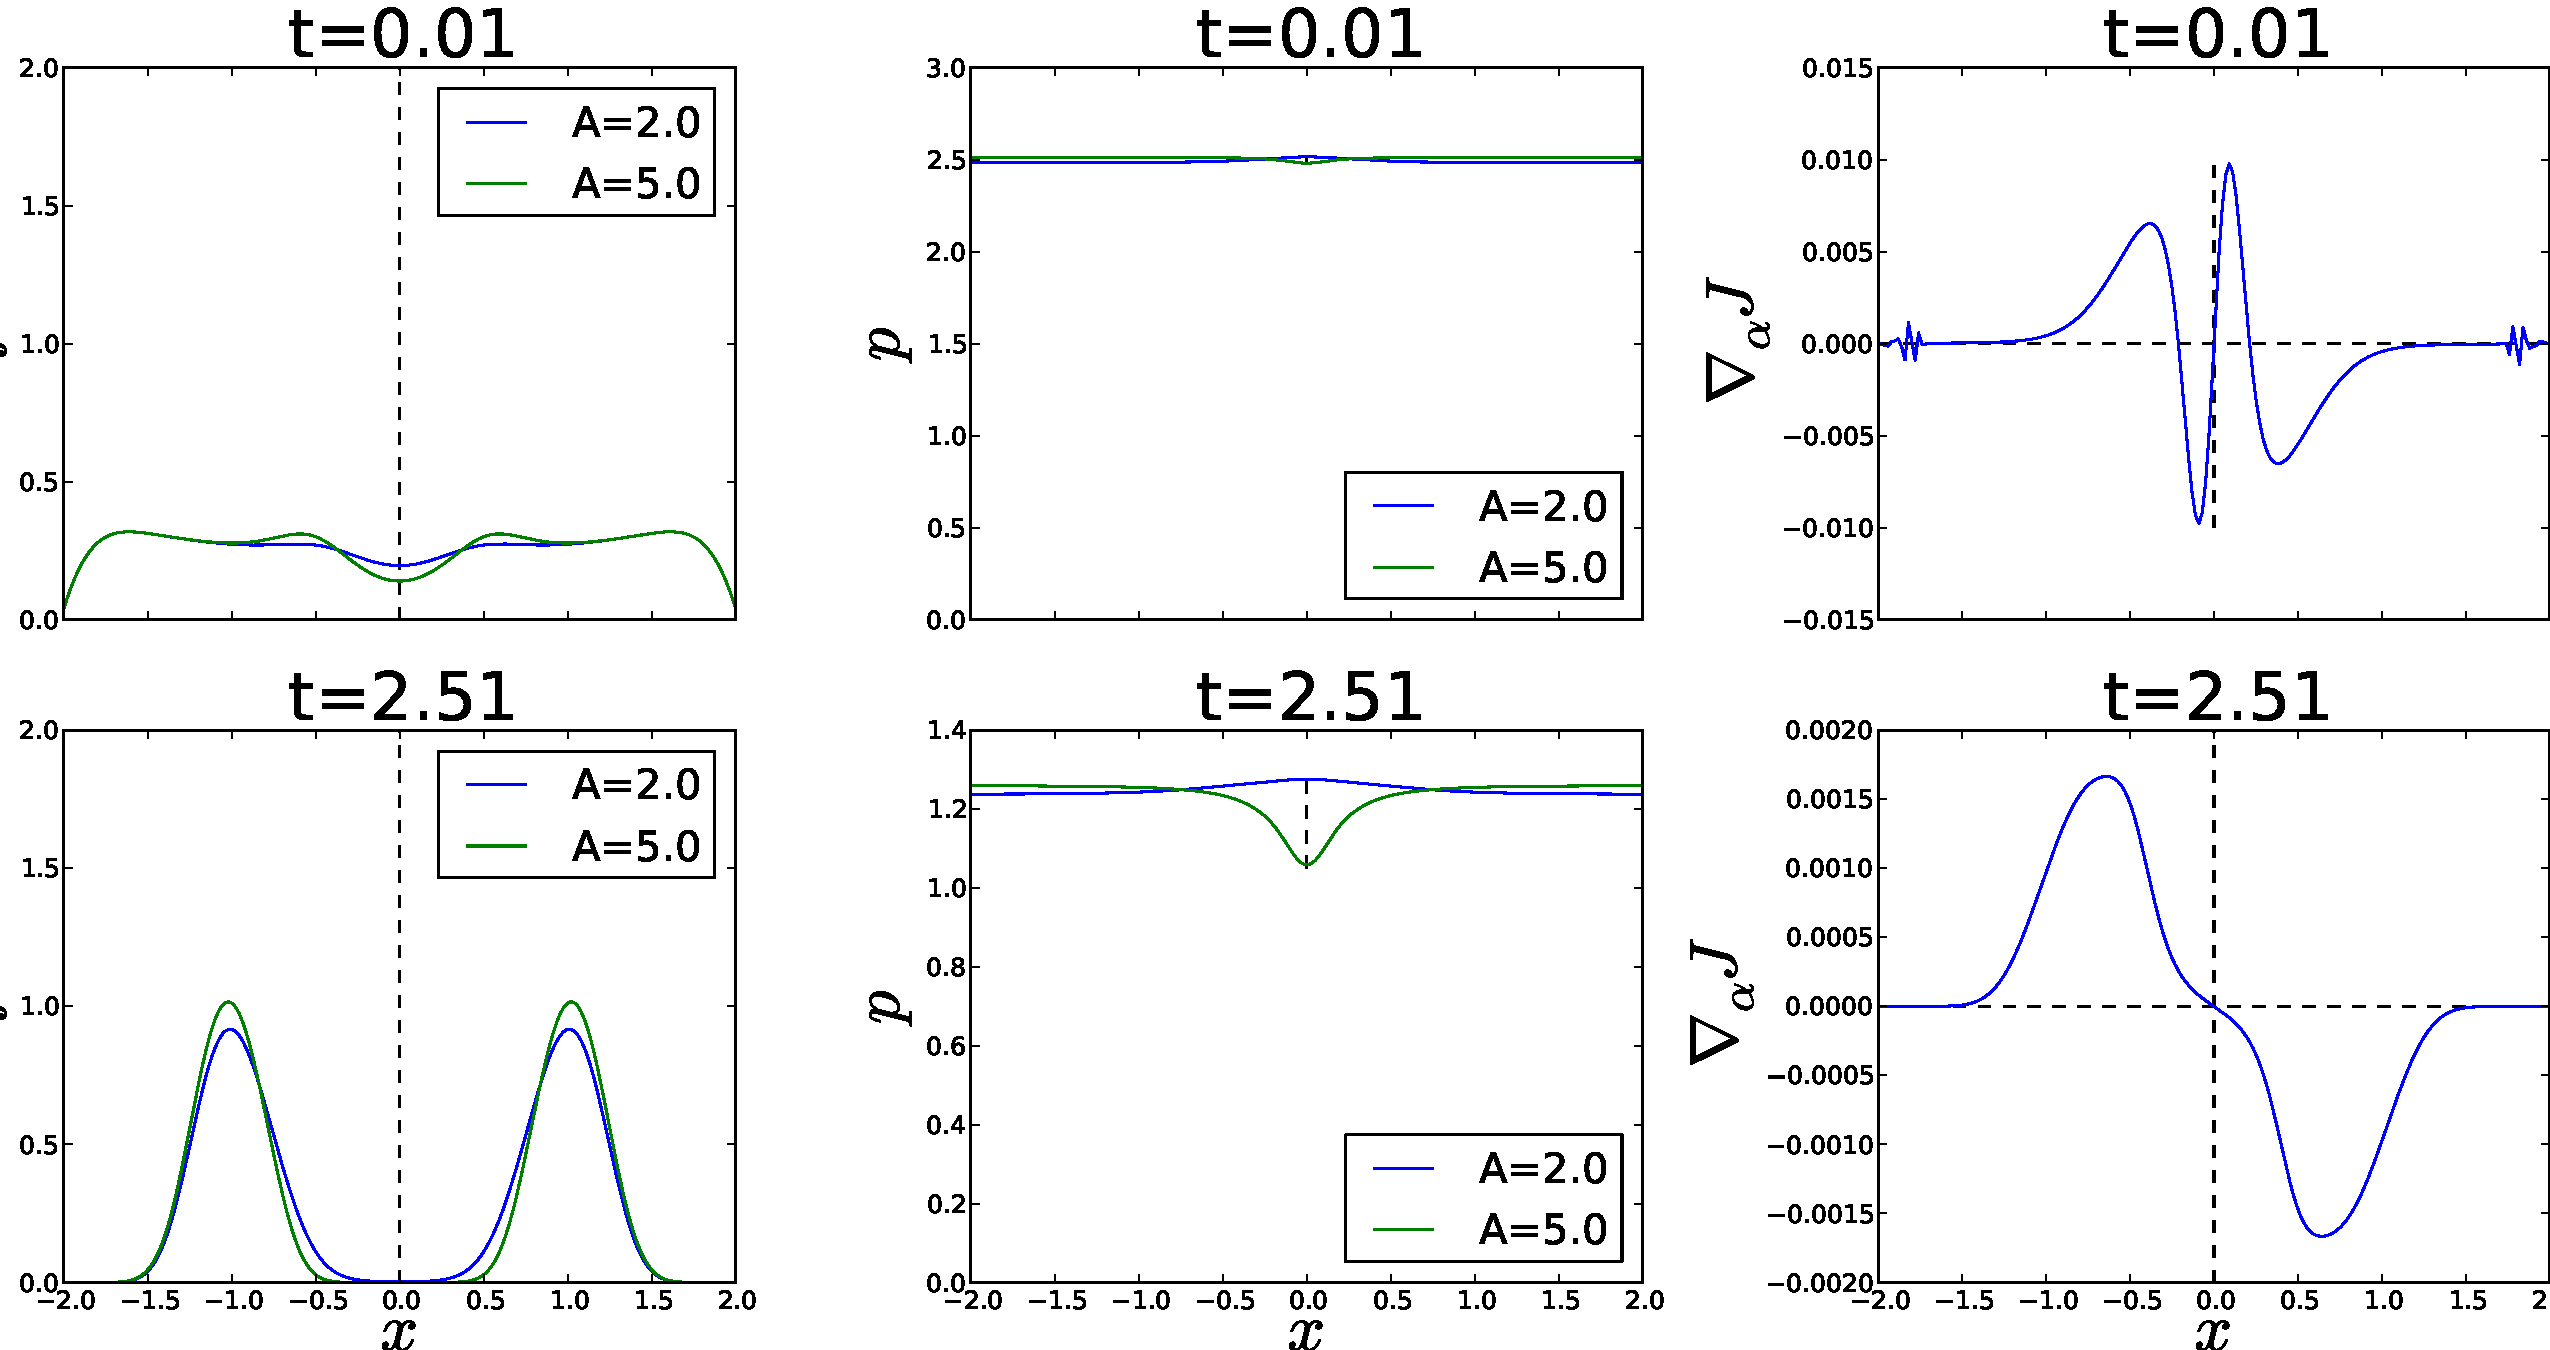
\includegraphics[width=.9\textwidth]{Figs/DoublewellFBSolver/FB_alpha_null_solution_2.pdf}
  \caption[labelInTOC]{Solution to the test Double Well potential problem using
  $\a \equiv 0$. }
  \label{fig:FBSoln_doublewell_alpha_null}
\end{center}
\end{figure} 

\end{frame}
\begin{frame}
% \frametitle{A more fair comparison}
\frametitle{Gradient Ascent (Kinda) Works} 
\begin{figure}[htp] 
\begin{center} 
  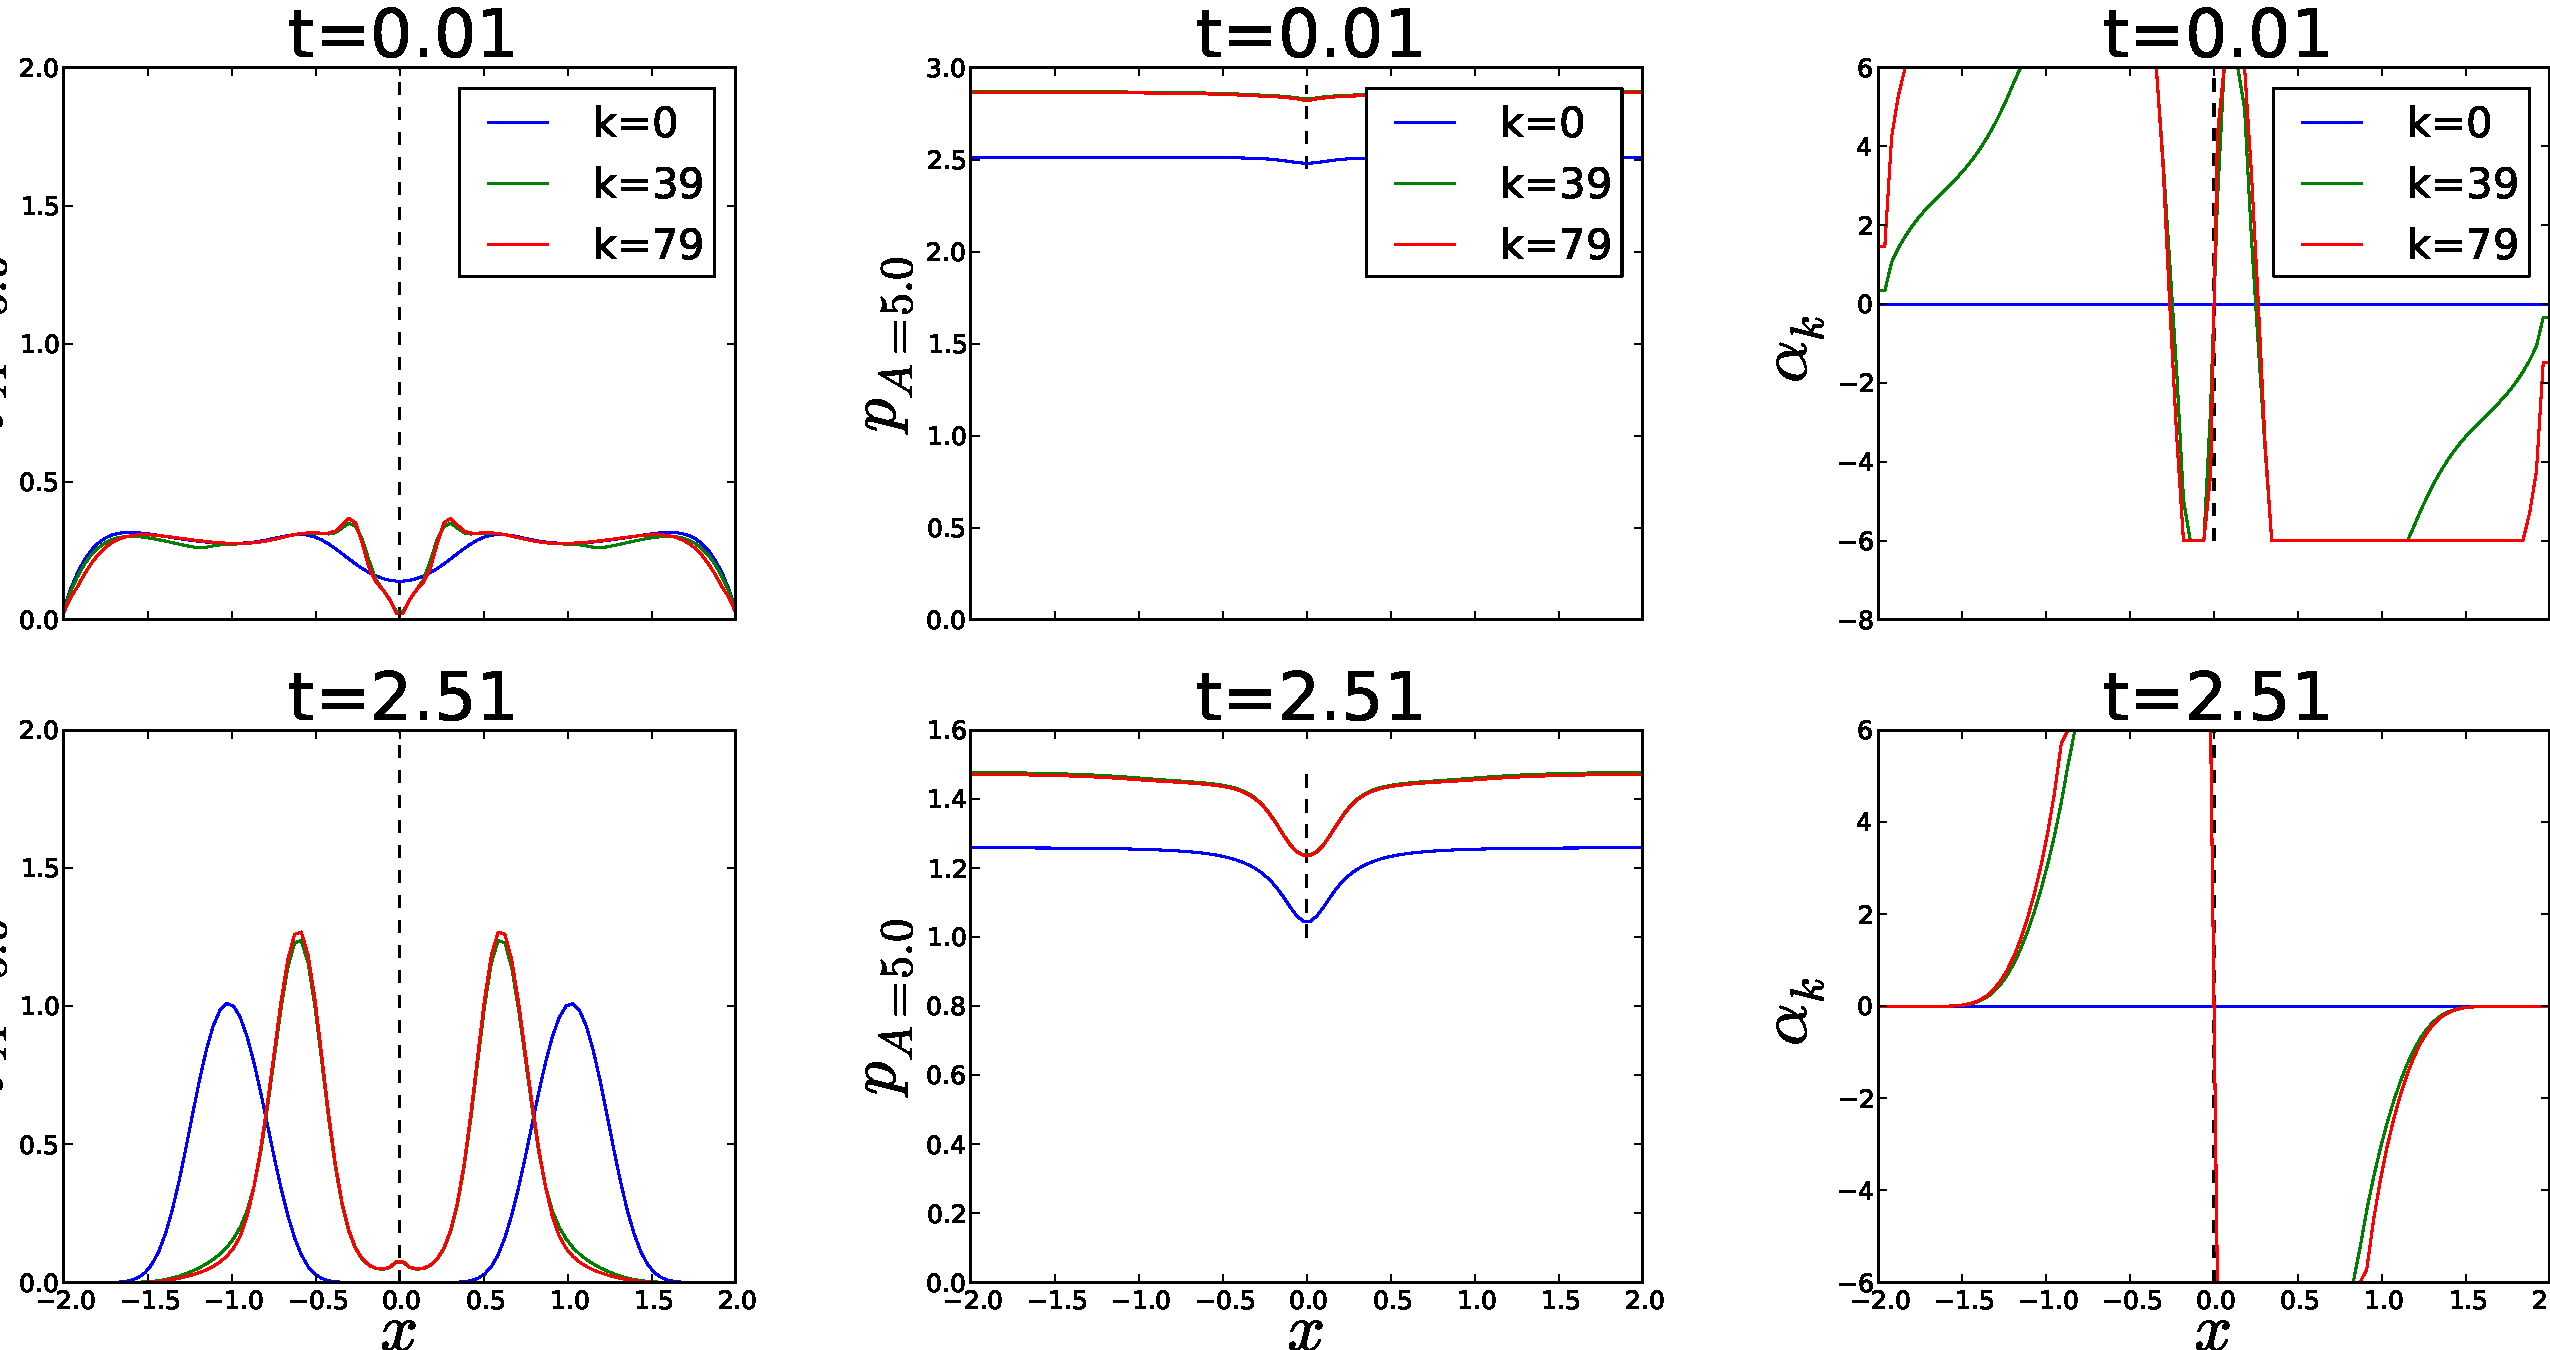
\includegraphics[width=.9\textwidth]{Figs/DoublewellFBSolver/FB_alpha_iterates_uICs_2.pdf}
  \caption[labelInTOC]{Solution to the test Double Well potential problem using
  $\a \equiv 0$. }
  \label{fig:FBSoln_doublewell_alpha_null}
\end{center}
\end{figure}
\end{frame}

\section*{Summary}

\begin{frame}
\frametitle<presentation>{Summary}
\begin{block}{SDE Optimal Design via the Mutual Information}
  \begin{itemize}
    \item Determine the maximally informative perturbation of an SDE using the
    criterion of Mutual Information between a belief distribution of the
    parameters and the forward density of the state trajectories
    \pause
    \item Use the Adjoint Method + a gradient ascent to
    obtain the optimal feedback-form perturbation  \pause
	\item Numerics of gradient-based optimization remain to
	be 'finessed'
  \end{itemize}
\end{block}

\vskip0pt plus.5fill
 \pause
\begin{block}{To be addressed:}
   \begin{itemize}
     \item More complex systems
     \item Higher dimensions 
     \item Obviate the need for PDE numerics (Stochastic Solution?)
   \end{itemize}
 \end{block}

\end{frame}

\end{document}
